\documentclass[border=10pt]{standalone}
\usepackage{tikz}
\usetikzlibrary{arrows.meta, positioning, calc, decorations.pathreplacing}
\usepackage{amsmath, amssymb}

% Colors
\definecolor{vblue}{RGB}{90,140,200}     % variable nodes
\definecolor{cred}{RGB}{200,75,60}       % check nodes
\definecolor{msggreen}{RGB}{60,160,90}   % messages
\definecolor{gy}{RGB}{105,105,105}       % gray labels
\definecolor{lbg}{RGB}{245,248,252}      % light background

\begin{document}
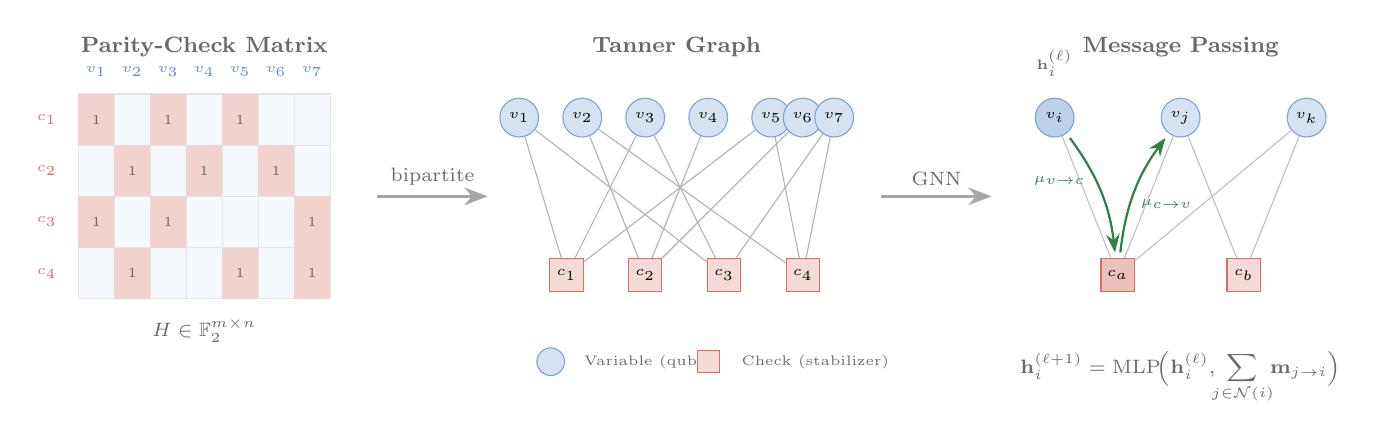
\begin{tikzpicture}[>=Stealth, font=\sffamily,
    vnode/.style={circle, draw=vblue!80, fill=vblue!25, minimum size=14pt,
                  inner sep=0pt, font=\tiny\bfseries},
    cnode/.style={rectangle, draw=cred!80, fill=cred!20, minimum size=12pt,
                  inner sep=0pt, font=\tiny\bfseries},
    msg/.style={->, thick, msggreen!80!black, shorten >=2pt, shorten <=2pt},
    lbl/.style={font=\scriptsize, gy}]

% ════════════════════════════════════════
%  LEFT: Parity-Check Matrix H
% ════════════════════════════════════════

\node[font=\footnotesize\bfseries, gy] at (1.6, 5.2) {Parity-Check Matrix};

% Matrix grid
\begin{scope}[shift={(0, 2.0)}]
    % Background
    \fill[lbg] (0,0) rectangle (3.2, 2.6);
    \draw[black!20] (0,0) rectangle (3.2, 2.6);

    % Grid lines
    \foreach \y in {0, 0.65, 1.3, 1.95, 2.6} {
        \draw[black!10] (0,\y) -- (3.2,\y);
    }
    \foreach \x in {0, 0.457, 0.914, 1.371, 1.828, 2.285, 2.742, 3.2} {
        \draw[black!10] (\x,0) -- (\x,2.6);
    }

    % Non-zero entries (1s) as filled cells
    % Row 0 (check c1)
    \fill[cred!25] (0.0,1.95) rectangle (0.457,2.6);
    \fill[cred!25] (0.914,1.95) rectangle (1.371,2.6);
    \fill[cred!25] (1.828,1.95) rectangle (2.285,2.6);
    % Row 1 (check c2)
    \fill[cred!25] (0.457,1.3) rectangle (0.914,1.95);
    \fill[cred!25] (1.371,1.3) rectangle (1.828,1.95);
    \fill[cred!25] (2.285,1.3) rectangle (2.742,1.95);
    % Row 2 (check c3)
    \fill[cred!25] (0.0,0.65) rectangle (0.457,1.3);
    \fill[cred!25] (0.914,0.65) rectangle (1.371,1.3);
    \fill[cred!25] (2.742,0.65) rectangle (3.2,1.3);
    % Row 3 (check c4)
    \fill[cred!25] (0.457,0.0) rectangle (0.914,0.65);
    \fill[cred!25] (1.828,0.0) rectangle (2.285,0.65);
    \fill[cred!25] (2.742,0.0) rectangle (3.2,0.65);

    % 1s text
    \node[font=\tiny,gy] at (0.228,2.275) {1};
    \node[font=\tiny,gy] at (1.142,2.275) {1};
    \node[font=\tiny,gy] at (2.056,2.275) {1};
    \node[font=\tiny,gy] at (0.685,1.625) {1};
    \node[font=\tiny,gy] at (1.599,1.625) {1};
    \node[font=\tiny,gy] at (2.513,1.625) {1};
    \node[font=\tiny,gy] at (0.228,0.975) {1};
    \node[font=\tiny,gy] at (1.142,0.975) {1};
    \node[font=\tiny,gy] at (2.971,0.975) {1};
    \node[font=\tiny,gy] at (0.685,0.325) {1};
    \node[font=\tiny,gy] at (2.056,0.325) {1};
    \node[font=\tiny,gy] at (2.971,0.325) {1};

    % Row labels (checks)
    \node[font=\tiny, cred!80, anchor=east] at (-0.15, 2.275) {$c_1$};
    \node[font=\tiny, cred!80, anchor=east] at (-0.15, 1.625) {$c_2$};
    \node[font=\tiny, cred!80, anchor=east] at (-0.15, 0.975) {$c_3$};
    \node[font=\tiny, cred!80, anchor=east] at (-0.15, 0.325) {$c_4$};

    % Column labels (variables)
    \node[font=\tiny, vblue, anchor=south] at (0.228, 2.7) {$v_1$};
    \node[font=\tiny, vblue, anchor=south] at (0.685, 2.7) {$v_2$};
    \node[font=\tiny, vblue, anchor=south] at (1.142, 2.7) {$v_3$};
    \node[font=\tiny, vblue, anchor=south] at (1.599, 2.7) {$v_4$};
    \node[font=\tiny, vblue, anchor=south] at (2.056, 2.7) {$v_5$};
    \node[font=\tiny, vblue, anchor=south] at (2.513, 2.7) {$v_6$};
    \node[font=\tiny, vblue, anchor=south] at (2.971, 2.7) {$v_7$};
\end{scope}

\node[font=\scriptsize, gy] at (1.6, 1.6) {$H \in \mathbb{F}_2^{m \times n}$};

% ════════════════════════════════════════
%  ARROW: Matrix → Graph
% ════════════════════════════════════════

\draw[->, very thick, black!35] (3.8, 3.3) -- node[above, font=\scriptsize, gy] {bipartite} (5.2, 3.3);

% ════════════════════════════════════════
%  MIDDLE: Tanner Graph
% ════════════════════════════════════════

\node[font=\footnotesize\bfseries, gy] at (7.6, 5.2) {Tanner Graph};

% Variable nodes (top row)
\node[vnode] (v1) at (5.6, 4.3) {$v_1$};
\node[vnode] (v2) at (6.4, 4.3) {$v_2$};
\node[vnode] (v3) at (7.2, 4.3) {$v_3$};
\node[vnode] (v4) at (8.0, 4.3) {$v_4$};
\node[vnode] (v5) at (8.8, 4.3) {$v_5$};
\node[vnode] (v6) at (9.2, 4.3) {$v_6$};
\node[vnode] (v7) at (9.6, 4.3) {$v_7$};

% Check nodes (bottom row)
\node[cnode] (c1) at (6.2, 2.3) {$c_1$};
\node[cnode] (c2) at (7.2, 2.3) {$c_2$};
\node[cnode] (c3) at (8.2, 2.3) {$c_3$};
\node[cnode] (c4) at (9.2, 2.3) {$c_4$};

% Edges (matching the H matrix)
\draw[black!30] (v1) -- (c1);
\draw[black!30] (v3) -- (c1);
\draw[black!30] (v5) -- (c1);
\draw[black!30] (v2) -- (c2);
\draw[black!30] (v4) -- (c2);
\draw[black!30] (v6) -- (c2);
\draw[black!30] (v1) -- (c3);
\draw[black!30] (v3) -- (c3);
\draw[black!30] (v7) -- (c3);
\draw[black!30] (v2) -- (c4);
\draw[black!30] (v5) -- (c4);
\draw[black!30] (v7) -- (c4);

% Legend
\node[vnode, minimum size=10pt] at (6.0, 1.2) {};
\node[font=\tiny, gy, anchor=west] at (6.3, 1.2) {Variable (qubit)};
\node[cnode, minimum size=8pt] at (8.0, 1.2) {};
\node[font=\tiny, gy, anchor=west] at (8.3, 1.2) {Check (stabilizer)};

% ════════════════════════════════════════
%  ARROW: Graph → GNN
% ════════════════════════════════════════

\draw[->, very thick, black!35] (10.2, 3.3) -- node[above, font=\scriptsize, gy] {GNN} (11.6, 3.3);

% ════════════════════════════════════════
%  RIGHT: GNN Message Passing
% ════════════════════════════════════════

\node[font=\footnotesize\bfseries, gy] at (14.0, 5.2) {Message Passing};

% Variable nodes
\node[vnode, fill=vblue!40] (gv1) at (12.4, 4.3) {$v_i$};
\node[vnode] (gv2) at (14.0, 4.3) {$v_j$};
\node[vnode] (gv3) at (15.6, 4.3) {$v_k$};

% Check nodes
\node[cnode, fill=cred!35] (gc1) at (13.2, 2.3) {$c_a$};
\node[cnode] (gc2) at (14.8, 2.3) {$c_b$};

% Edges
\draw[black!25] (gv1) -- (gc1);
\draw[black!25] (gv2) -- (gc1);
\draw[black!25] (gv2) -- (gc2);
\draw[black!25] (gv3) -- (gc1);
\draw[black!25] (gv3) -- (gc2);

% Message arrows (green, showing flow)
\draw[msg, bend left=15] (gv1) to
    node[left, font=\tiny, msggreen!80!black, pos=0.4] {$\mu_{v \to c}$} (gc1);
\draw[msg, bend left=15] (gc1) to
    node[right, font=\tiny, msggreen!80!black, pos=0.4] {$\mu_{c \to v}$} (gv2);

% Node feature annotation
\node[font=\tiny, gy, align=center, anchor=south] at (12.4, 4.7)
    {$\mathbf{h}_i^{(\ell)}$};

% Update equation
\node[font=\scriptsize, gy, align=center] at (14.0, 1.0)
    {$\mathbf{h}_i^{(\ell+1)} = \mathrm{MLP}\!\Big(\mathbf{h}_i^{(\ell)},
      \!\!\displaystyle\sum_{j \in \mathcal{N}(i)}\!\! \mathbf{m}_{j \to i}\Big)$};

\end{tikzpicture}
\end{document}
